\chapter{Conception détaillée}

\section*{Introduction}
Le dernier pas dans la conception de notre logiciel est de spécifier en détails tous les composants et leur rôles. Nous aurons de ce fait décrit tous les aspects de notre programme et pourrons le développer sans ambiguïtés.

\section{Répertoire de décisions}

Mais avant de rentrer dans les détails de la conception, nous devons préciser les modifications apporter au modèle durant le développement.\\
Pour rappel, le modèle après analyse était la figure \ref{ddcanalyse}.

\begin{figure}[!ht]
\begin{center}
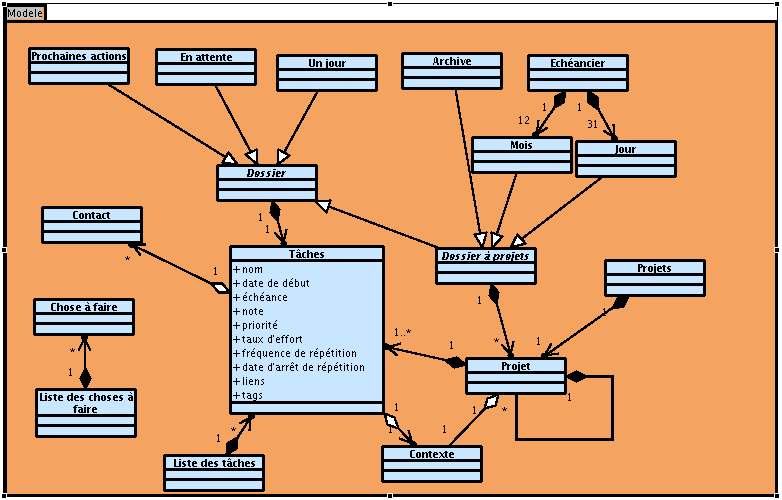
\includegraphics[width=12cm]{images/DiagrammedeClasse.png}
\caption{Diagramme de classes du modèle après analyse}
\label{ddcanalyse}
\end{center}
\end{figure}

Et maintenant, le diagramme de classe est représenté par la figure \ref{ddcfinal}.

\begin{figure}[!ht]
\begin{center}
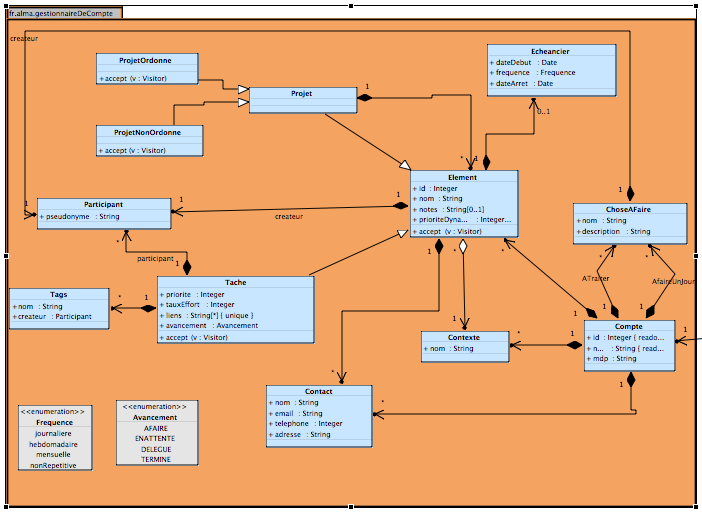
\includegraphics[width=12cm]{images/ClassDiagram.png}
\caption{Diagramme de classes du modèle à la fin du projet}
\label{ddcfinal}
\end{center}
\end{figure}


Les modifications sont nombreuses :
\begin{itemize}
\item Suppression de la classe Mois (Les échéances sont stockées dans l'échéancier et les tâches ou projets qui l'utilisent pointent dessus);
\item Suppression de la classe Jour (comme Mois);
\item Suppression de Archive (les éléments contiennent un état pour renseigner si ils sont actifs ou non);
\item Suppression des "dossiers" Dossier/Dossier à projets/Projets (la version informatique rend obsolète l'utilisation de dossiers);
\item Suppression de Prochaines Actions (élément visuel, les tâches sont afficher en fonction des choix de l'utilisateur);
\item Suppression de Liste des Tâches (affichage des tâches, pas besoin de les stocker ensemble);
\item Modification de Liste des Choses à faire (attribut d'une autre classe);
\item Modification de Contacts et Tags (ajout d'attributs);
\item Modification de En Attente (contenu dans l'état de l'élément);
\item Modification de Un Jour (attribut d'une autre classe);
\item Ajout de Participants (nécessaire pour les éléments ordonnés et connaître les dépendances);
\item Ajout de Projet Ordonné et de Projet Non Ordonné (sous classes de Projet);
\item Ajout de Éléments (pour regrouper les attributs commun de Tâche et Projet, et implémenter le patron Composition)
\item Ajout de Compte (contient toutes les autres classes).
\end{itemize}

Ainsi nous obtenons le diagramme de classe de la figure \ref{ddcfinal} et pouvons ainsi commencer la conception détaillée.

\section{Diagrammes statiques et dynamiques}

Le diagramme de classe du modèle n'est pas le seul à avoir changé, le reste du diagramme de classe a lui aussi eu des modifications(Voir figure \ref{ddctotal}).

\begin{figure}[!ht]
\begin{center}
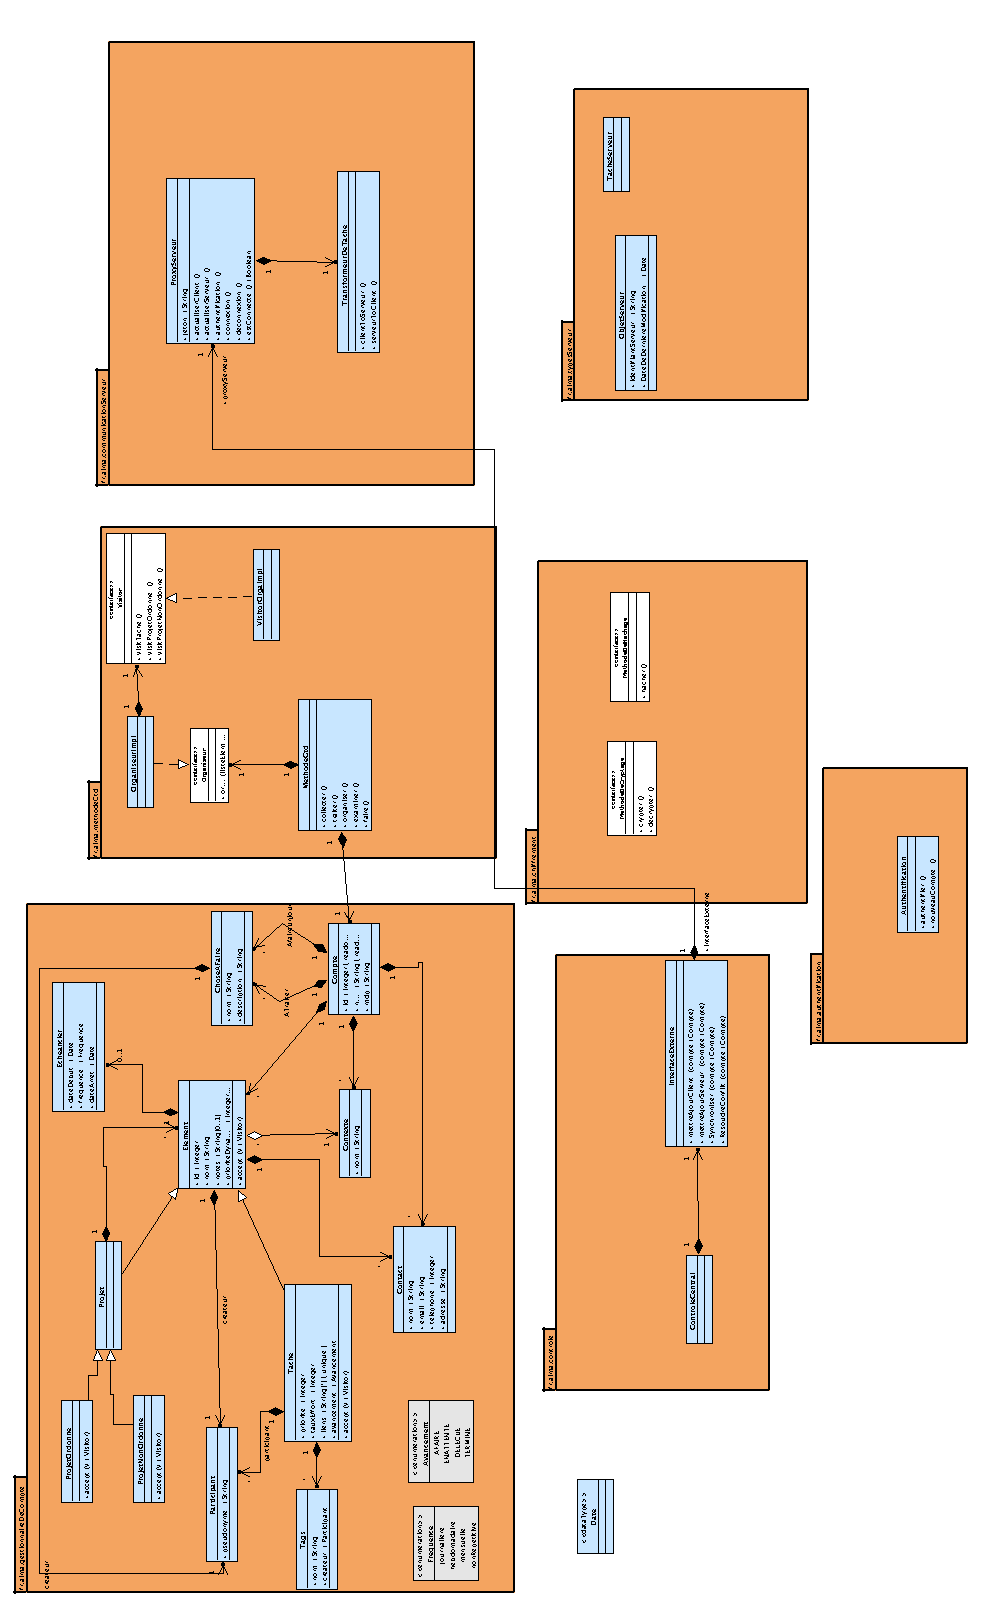
\includegraphics[width=14cm]{images/FullClassDiagram.png}
\caption{Diagramme de classes final}
\label{ddctotal}
\end{center}
\end{figure}

On peut voir les différentes interactions entre les composants décrits dans le chapitre "Spécification des Composants".


\section{Spécification des classes}

Cette section comporte une liste de toutes les classes en spécifiant pour chacune d'elles ses invariants.\\


\subsection*{Package : Gestionnaire de Compte}

\subsubsection*{Classe : Compte} 
\begin{itemize}
\item Nom jamais vide
\item Mot de passe jamais vide
\end{itemize}


\subsubsection*{Classe : Chose A Faire}
\begin{itemize}
\item Nom jamais vide
\item description jamais vide
\end{itemize} 

\subsubsection*{Classe : Contexte}
\begin{itemize}
\item Nom jamais vide
\end{itemize} 

\subsubsection*{Classe : Contact}
\begin{itemize}
\item Le couple nom/adresse unique
\item Nom jamais vide
\item Adresse jamais vide
\end{itemize} 

\subsubsection*{Classe : Élément}
\begin{itemize}
\item Nom jamais vide
\end{itemize} 

\subsubsection*{Classe : Participant}
\begin{itemize}
\item Id unique
\item Pseudonyme jamais vide
\end{itemize} 

\subsubsection*{Classe : Échéancier}
\begin{itemize}
\item Triplet d'attributs unique
\end{itemize}

\subsubsection*{Classe : Tag}
\begin{itemize}
\item Nom non vide
\item Nom unique
\end{itemize}

\section*{Conclusion}
Toutes les étapes de l'analyse étant terminées, nous pouvons finalement commencé l'implémentation qui est facilitée grâce à l'analyse poussée que nous avons réalisé. La génération de code à partir de notre modèle nous fera gagner du temps et l'utilisation de frameworks, tels Hibernate, nous facilitera la tâche.